%\documentclass[aps,preprint,amsmath,amssymb]{revtex4-1}% APS journal style
\documentclass[aps,reprint,amsmath,amssymb,prl]{revtex4-1}% APS journal style
\usepackage{graphicx}% Include figure files
\usepackage{dcolumn}% Align table columns on decimal point
\usepackage{bm}% bold math
\usepackage{hyperref}% add hypertext capabilities
%\bibliography{natbib}

\begin{document}
\title{A toy model to understand the dynamics of the vortical motions in turbulent boundary layers}
\author{J.C. Cuevas Bautista}
\email{jcc1@wildcats.unh.edu}
\affiliation{University of New Hampshire, Department of Mechanical Engineering, Durham 03824, USA.}
\date{\today}
\begin{abstract}
\noindent 
Recent studies indicate that the structure of the turbulent boundary layer at high Reynolds number (\textit{Re}) is composed of large uniform momentum zones segregated by fissures of concentrated vorticity. Experiments reveal that the dimensionless fissures thickness (scaled by boundary layer thickness) is $\mathcal{O}(1/\sqrt{Re})$ and the dimensionless streamwise velocity jump across a fissure scales with the friction velocity $\mathcal{O}(u_{\tau})$. A toy model that captures the essential elements of the turbulent boundary layer structure at high \textit{Re} is constructed to evaluate the long-time averaged flow statistics of the boundary layer. First, a ``master'' instantaneous  streamwise velocity profile in the wall-normal direction is constructed by placing a discrete number of fissuress across the boundary layer thickness. The number of fissures and their wall-normal locations follow scalings informed by the Mean Momentum Balance (MMB) theory. Next, the wall-normal positions of the fissures are allowed to randomly move in the wall-normal direction creating a statistically independent second instantaneous velocity profile. This process is then repeated to create an ensemble of instantaneous velocity profiles from which average statistics of the turbulent boundary layer can be computed and assessed. The statistics of the toy model are compared to statistics acquired in turbulent boundary layers at high \textit{Re}.
%Turbulent boundary layers are the result of complex interactions between a wide variety of scales present in the flow. Recent investigations indicates that the structure of turbulent boundary layers are physically composed of large uniform momentum zones segregated by fissures of concentrated vorticity which thickness scales with the Reynolds number $\delta^+$ as $1/\sqrt{\delta^+}$. The simplified model presented in this paper pretend to explain how these vortical fissures populate the turbulent boundary layer in special the inertial region. To do this Reynolds-Averaged Navier-Stokes equations must be simplified and solved, however in this model an alternative approach is considered. The thickness of vortical fissures is assumed negligible and the streamwise mean velocity profile is simulated as the result of the ensemble average of the instantaneous step velocity profiles. In addition the step profiles are modelled by zones of uniform velocity with discontinuous jumps of velocity (vortical fissures) along the wall normal position. Finally the positions of the vortical fissures are computed based on the Mean Momentum Balance theory (MMB) likewise the velocity increments. Results are computed for different Reynolds numbers and freestream velocities. The accurateness of the model is verified comparing the statistics of the first four moments of the turbulent mean velocity profile with the respective moments of the experimental data.
\end{abstract}
\keywords{turbulent boundary layer, uniform momentum zones, vortical fissures and Mean Momentum Balance theory.}
%Words=207.
\maketitle
\section{Numerical Methods}
A stream-wise master velocity profile is represented by a set of discrete steps uniformly spaced according with Eqs.~\ref{eq:upvel} and ~\ref{eq:yppos}, 
\begin{align}
U^+_{i+1}=&U^+_i+\phi_c^2 ln(\phi_c) \label{eq:upvel},\\
y^+_{i+1}=&\phi_c y^+_i \label{eq:yppos}.
\end{align}
These relationships are  derived from the MMB theory~\citep{Klewickimmb}, where Eq.~\ref{eq:upvel} determine the increments in the stream-wise normalized velocity $U^+$, the width of the steps in the $x$ coordinate and
Eq.~\ref{eq:yppos} determine the increments in the normalized wall normal position $y^+$, the height of the steps in the y coordinate (See Fig.~\ref{fig:master_profile}). The initial wall normal position was set to $y^+_0=100$ in order to coincide with the boundary edge of the log-layer in the traditional law-wall theory and $U^+_0=0.5 U_{\infty}^+$ to be the half of the free-stream velocity. The constant factor $\phi_c$ is given by $\phi_c=(1+\sqrt{5})/2$ and since the thickness of the
vortical fissures scales like $\mathcal{O}(1/\sqrt{Re})$, it is considered negligible for this model.  Using the information described above a master profile is constructed, the input parameters are the Reynolds number associated with the boundary layer thickness

\begin{equation}\label{eq:deltap}
\delta^+=\frac{\delta}{\nu/u_{\tau}},
\end{equation}
where $u_{\tau}=\sqrt{\tau_{\omega}/\rho}$ is the friction velocity ($\tau_{\omega}$ is the mean wall shear stress and $\rho$ is the mass density respectively) and $U^+_{\infty}$. 
Fig.~\ref{fig:master_profile} 
\begin{figure}[b]
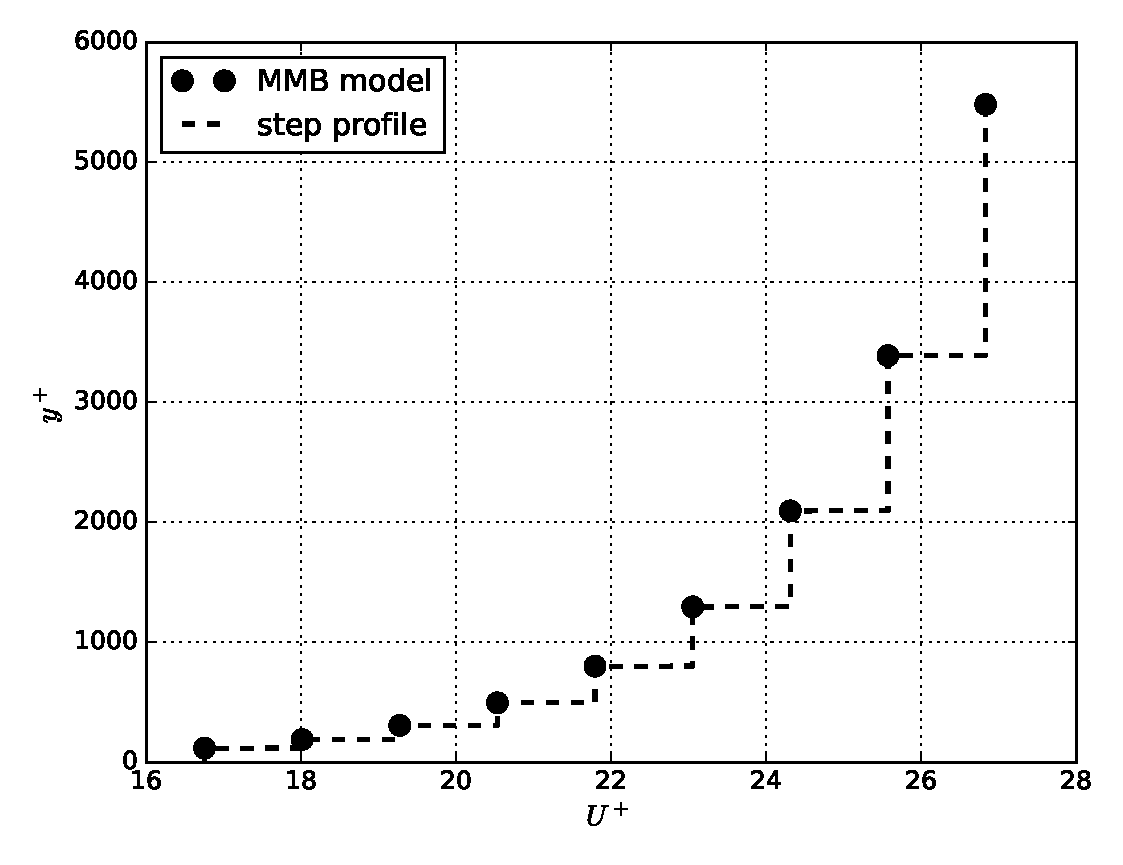
\includegraphics[scale=0.46]{figures/Master_step_profile}
\caption{\label{fig:master_profile} Step turbulence master profile for $\delta^+=5200$ and $U^+_{\infty}=26.5$.}
\end{figure} 
depicts the step turbulent master profile with a grid of $5481$ linearly spaced points in the wall normal direction each one associated to a velocity. The dot circles are the positions of the vortical fissures computed using Eqs.~\ref{eq:yppos} and \ref{eq:upvel} respectively. The zones of uniform momentum are created assigning the same velocity of the vortical fissure to the grid points spanned between previous vortical fissure and the actual vortical fissure. Thus the number of vortical fissures dictates the number of uniform momentum zones. The instantaneous multiple velocity profiles are created by add a gaussian perturbation of the actual height to the positions of the vortical fissures (Black dots in Fig.~\ref{fig:master_profile}) in the step turbulent master profile. Once the new wall normal positions for the vortical fissures are obtained the grid is filled with uniform momentum zones similarly to the process described above. Fig.~\ref{fig:mul_profiles} shows five instantaneous turbulent velocity profiles, it can be seen how the vortical fissures changes their position trough the boundary layer for the different profiles, the time units are arbitrary, i.e. they just illustrate different instants of time. These vortical fissure are allowed to change their positions with their respective associated velocity, this physically means that the vortical fissures can cross each other in the turbulent boundary layer  profile generating zones of negative vorticity.
\begin{figure}[b]
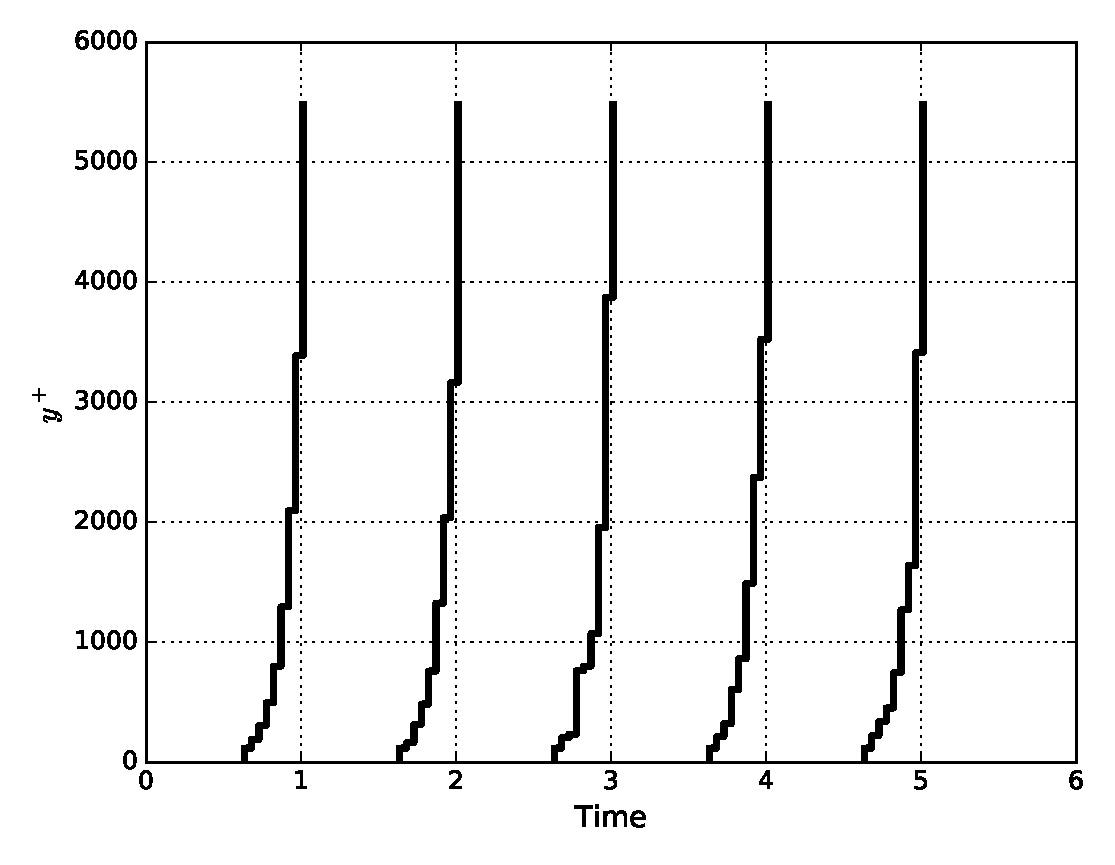
\includegraphics[scale=0.46]{figures/multiple_instantaneous_vprof}
\caption{\label{fig:mul_profiles} Multiple instantaneous velocity profiles with a gaussian perturbation of mean $\mu=0$ and standard deviation $\sigma=0.4$.}
\end{figure}
The multiple instantaneous velocity profiles are independent each other, thus to create statistically consistency 5000 independent realizations were created and averaged. As a consequence a mean turbulent profile is created (See Fig.~\ref{fig:mean_profile}).
\begin{figure}[b]
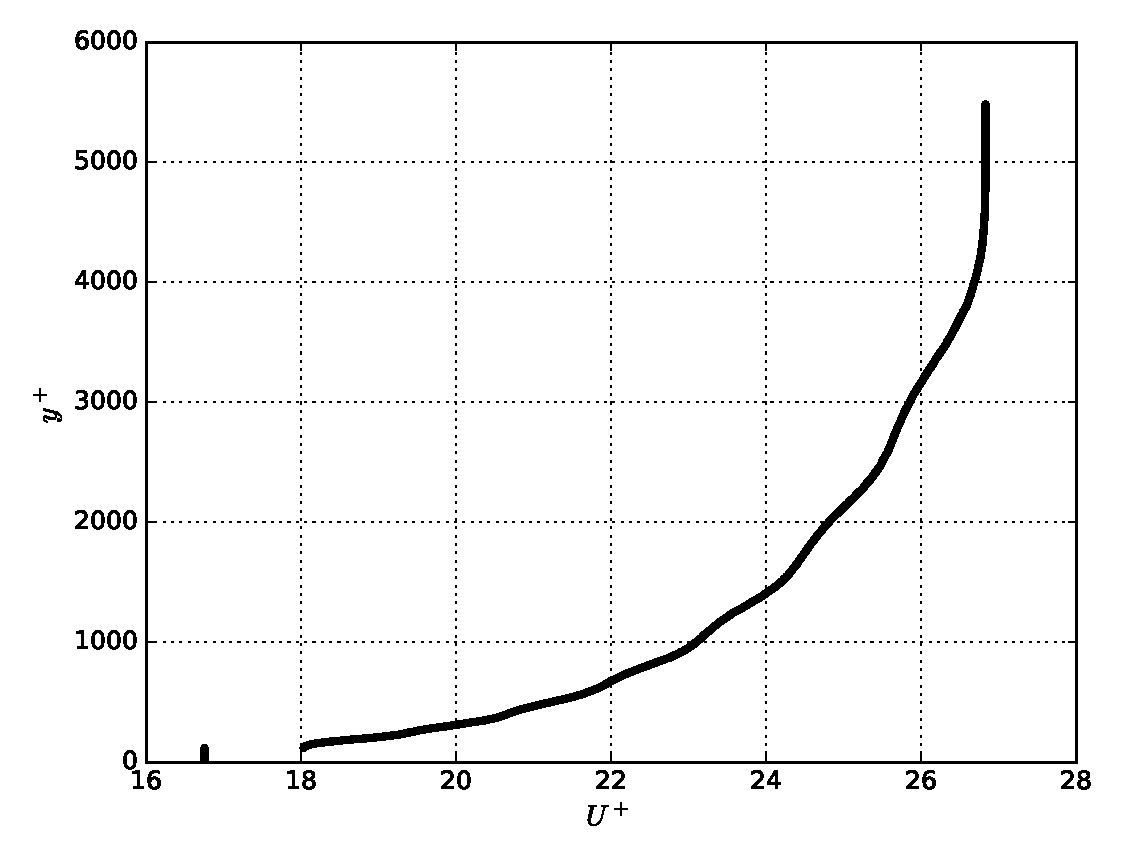
\includegraphics[scale=0.46]{figures/Master_averaged_step_profile_5000_assembles}
\caption{\label{fig:mean_profile} Mean turbulent stream-wise velocity profile for 5000 independent realizations with a gaussian perturbation of $\mu=0$ and $\sigma=0.4$.}
\end{figure} 


\bibliography{Aps_template}% Produces the bibliography via BibTeX.
\end{document}
